\section{Prototypen}
\label{prototypen}

Vår prototype, som er vårt forslag til forbedringene vi kom frem til gjennom literaturstudiene, og som ble test gjennom to workshops, er basert på bruk av smarttelefon, i motsettning til telefonene fra cisco som er i bruk i dag. Grunnen til dette valget ligger i at dette er mer fremtidsrettet og gir bedre mulighet for mer utfyllende informasjon i skjermbildet, samtidig som det også gir mulighet for interaksjon med brukeren og åpner for å senere legge til funksjunalitet som eksempelvis å hente frem annen informasjon, som journaler og prøvesvar. Vi har etterstebet å lage et intuitivt design, som gir god informasjon for å støtte awareness.

\noindent
Applikasjonen er tenkt å være den eneste kjørende på telefonen, hvor vanlige funksjoner som telefon er inkludert, slik at det kun er denne applikasjonen som brukes - også for vanlige telefonsamtaler. Vi vil i de neste delene gi en forklaring på prtotypens design og funksjonalitet. Da dagens pasientsignal-system er beskrevet i appendiks \ref{appendix_dagenssystem} vil vi oppfordre leserene til å lese dette appendikset ved uklarheter rundt systemets oppbyggning og funksjonalitet.

\noindent
En antagelse som er gjort er at det er implementert systemer for lokalisering av sykepleierene, slik at systemet kan vite hvilket rom sykepleierene er i til en hver tid. Denne funksjonen vil bli brukt av statusindikatoren beskrevet senere i dette kapittelet. Bardram (2004) trekker frem at mange sykepleiere er skeptiske til slik sporing, med begrunnelse i at det i ettertid kan lages statistikker på hvor lenge man er hvor, som blandt annet på pauserommet. Vårt forslag er å ikke lagre denne informasjonen i det hele tatt, slik at den heller ikke kan brukes mot sykepleierene i ettertid. I forhold til systemet har informsjonen kun verdi i sanntid, og det er derfor ingen grunn til å lagre denne informsjonen.

\noindent
Presentasjon av pasientsignalet, formidling av sykepleierenes tilgjengelighet og spesielt kombinasjonen av disse har vært vårt hovedfokus i utviklingen av denne prototypen. Det er derfor også disse som er lagt mest vekt på i dette kapittelet. De øvrige fonksjonene og skjermbildene er med for å skape et helhetlig inntrykk av prototypen, og for å hjelpe deltagerene på workshoppene til å se muligheter og komme på egne ideer til hva de mener vil være nyttig funksjonalitet og informasjon.

\subsection{Tilgjengelighet og pasientsignal}
Disse to er tett knyttet sammen for å assistere sykepleierene i valget om de skal godta eller avvise et pasientsignal. Kunnskap om kollegers tilgjengelighet kan også legges til grunn ved avgjørelser angående om, og hvordan, man skal ta kontakt med andre sykepleiere. Teorien som er lagt til grunn for valgene vi har gjort her er presentert i \ref{chp: kognisjon}, \ref{chp: awareness} og \ref{chp: avbrudd}.

\subsubsection{Tilgjengelighet}
Tilgjengelighet-indikatoren har som formål å fortelle sykepleieren om hvilken tilgjengelighet han/hun er satt som for øyeblikket. Vi har valgt å bruke tre forskjellige statuser; "tilgjengelig"\ (grønn), "på rom"\ (gul), og "opptatt"\ (rød) (figur \ref{tilgjengelighetsstatuser}). Denne er i utgangspunktet satt som tilgjengelig. Når sykepleieren går inn på et rom vil denne automatisk skiftes til "på rom", og motsatt når sykepleieren forlater rommet og går ut på gangen/tunet igjen. Dersom sykepleieren vet at oppgaven som skal utføres vil ta lang tid, og han/hun helst ikke vil forstyrres i løpet av denne tiden, kan statusen manuelt settes til "opptatt". Dette signaliserer til de andre sykepleierene at dersom det er mulig, skal en unngå å kontakte denne sykepleieren, da det vil forårsake en uønsket forstyrrelse. Denne statusen vil bli stående til sykepleieren igjen endrer status til "tilgjengelig". Eventuelt kan det gis en påminnelse etter en fastsatt tid som spør sykepleieren om det er meningen at statusen fremdeles skal være "opptatt". Teknologien som ligger bak denne automatikken er ikke en del av denne oppgaven.

\begin{figure}
	\centering
	\begin{subfigure}[b]{0.3\textwidth}
		
\includegraphics[scale=0.15]{statusGronn.jpg}
		\caption{Tilgjengelig}
		\label{proto_startside}
	\end{subfigure}
	\begin{subfigure}[b]{0.3\textwidth}
		
\includegraphics[scale=0.15]{statusGul.jpg}
		\caption{På rom}
		\label{proto_startside}
	\end{subfigure}
	\begin{subfigure}[b]{0.3\textwidth}
		
\includegraphics[scale=0.15]{statusRod.jpg}
		\caption{Opptatt}
		\label{proto_startside_medMeny}
	\end{subfigure}
	\caption{Tilgjengelighetsstatuser}
	\label{tilgjengelighetsstatuser}
\end{figure}

\subsubsection{Pasientsignal}
Dette er en av de største endringene fra dagens system, og en av hovedfunksjonene med tanke på vår oppgave. Eksempel på enhetene som er i bruk i dag er avbildet i figur [SETT INN REF], mens skjermbilde ved pasientanrop ved bruk av prototypen er avbildet i figur \ref{protoPasientsignal}. Den største endringen vi har gjort, borstestt fra design, er at det vises en liste over de neste sykepleierene, samt deres tilgjengelighet, som vil bli oppringt dersom sykepleieren velger i avvise anropet. Hensikten med denne listen er å tilgjengeliggjøre informasjon som kan gi sykepleieren bedre grunnlag for avgjørelsen i forhold til om anropet skal godtas eller avvises.

\begin{figure}[H]
\centering
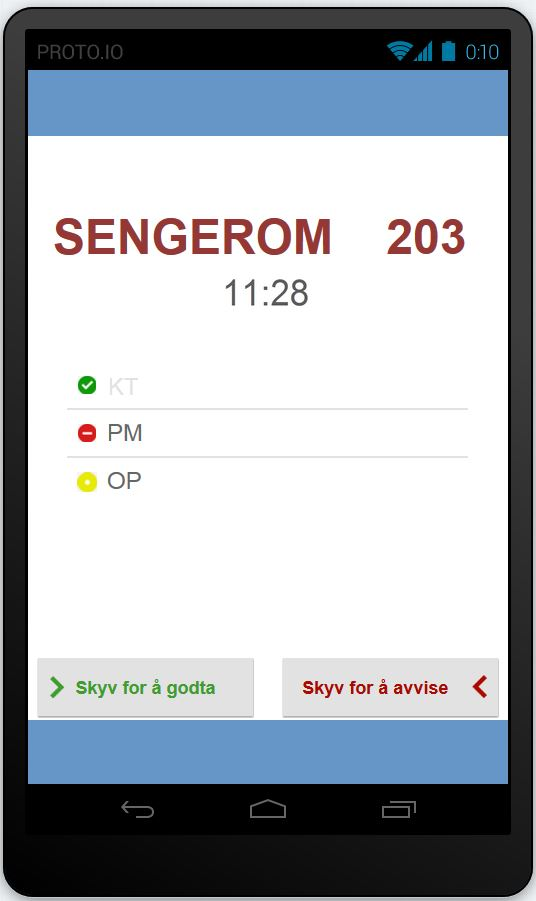
\includegraphics[scale=0.4]{proto_pasientsignal.jpg}
\caption{Skjermbilde ved inkommende pasientsignal. Her fra sengerom 203}
\label{protoPasientsignal}
\end{figure}

Med denne informsjonen umiddelbart tilgjengelig når en pasient ringer har sykepleieren mulighet til å, dersom han/hun ser at det er andre sykepleiere som er tilgjengelig, avvise anropet uten å være bekymret for at pasienten ikke får hjelp. Dette vil i andre omgang frigjøre kapasitet i arbeidsminnet (\ref{chp: kognisjon}) og dermed kan sykepleieren være mer mentalt tilstede hos pasienten som han/hun er hos på dette tidspunktet, som igjen gir bedre pasientomsorg.

\subsection{Skjermbildene og deres funksjon}

Som nevnt over er det paisentsignalet, og awareness-informsjonen som bilr kommunisert sammen med dette som er hovedfokuset i denne oppgaven. De øverige skjermbildene som her vil be presentert er laget av to grunner: de skal gi prototypen en mer helhetlig fremtoning, og de skal representere fremtidsrettet tankegang for fremtidig funksjonalitet, som kan være med å trigge kreativ tenkning hos deltagerene på workshoppene.

\subsubsection{Startsiden}
Forsiden er som ilustrert i figur \ref{proto_startside}. Knappen øverst til venstre gir tilgang til en dorp-down meny som vist i figur \ref{proto_startside_medMeny}. 

\begin{figure}[H]
	\centering
	\begin{subfigure}[b]{0.48\textwidth}
		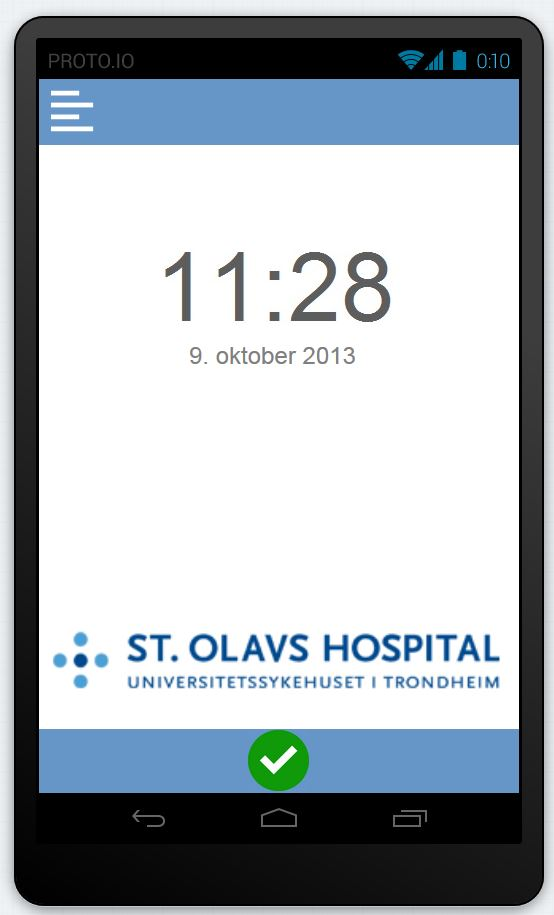
\includegraphics[scale=0.4]{proto_startside.jpg}
		\caption{Prototypens startside}
		\label{proto_startside}
	\end{subfigure}
	\begin{subfigure}[b]{0.48\textwidth}
		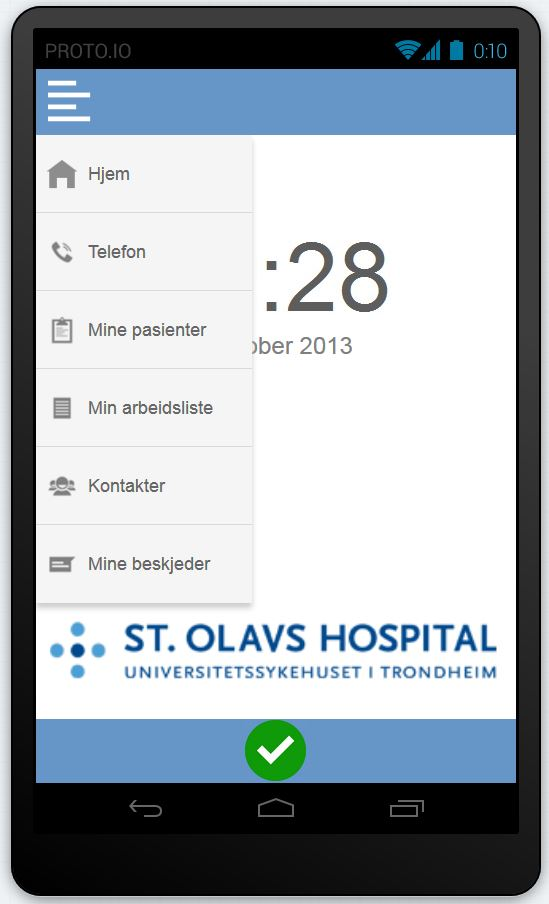
\includegraphics[scale=0.4]{proto_startside_medMeny.jpg}
		\caption{Prototypens startside med menyvisning}
		\label{proto_startside_medMeny}
	\end{subfigure}
	\caption{Prototypens startside}
\end{figure}

\noindent
Forsiden er ment som en standby-side, det vil si at det er denne siden som vises når skjermen slåes på. Tanken var at denne skal være enkel, med få elementer. Vi har derfor valgt kun klokke og datovisning i tillegg til status-indikatoren, midt på det nederste blå feltet (her illustrert med en grønn sirkel med hvit hake), og menyknappen øverst til venstre. Status-indikatoren og menyknappen vises på alle skjermbilder. 

\subsubsection{Min Arbeidsliste}
Her vises alle psientsignal du har godtatt, men ikke vært hos. Dette betyr at dersom du velger å godta et pasientsignal vil det legges i denne listen. Når du har gått inn på rommet hvor signalet ble utløst, vil elementet forsvinne fra listen. Dersom en sykepleier har godtatt flere psientsignal vil det da ligge flere elementer i listen. Dette er ment til å være til hjelp slik at sykepleieren ikke skal glemme noen av pasientene, selv om han/hun skulle bli avbrutt. Funksjonen vil på denne måten avlaste arbeidsminnet (se kapittel \ref{chp: kognisjon}) til sykepleierene slik at de kan være mer mentalt tilstede, og bedre kunne fokusere på oppgaven de holder på med.

\subsubsection{Mine Pasienter}
Dette er nok den funksjonen som er mest fremtidsrettet og åpen for mer informsjonsflyt slik prototypen står i dag. Sykepleierene fordeler pasientene mellom seg ved starten av hver vakt. Ved å registrere dette i bemanningsplanen (se appendiks \ref{appendix_dagenssystem}) vil disse legges i listen "Mine Pasienter". Her er ideen at det i fremtiden kunne være mulig å aksessere journaler, tidligere prøvesvar, samt få beskjed når nye prøvesvar er klare. Som vist i figur \ref{minePasienter}, kan nye blodprøvesvar da vasles og vises direkte på telefonen. Sykepleieren ser med én gang at det er kommet ny informasjon angående Hermansen. Ved å trykke på navnet hans ser man at varselet gjelder svar på blodprøvene, og ved å trykke på teksen "nye blodprøvesvar"\ vil svarene straks vises.

\begin{figure}[H]
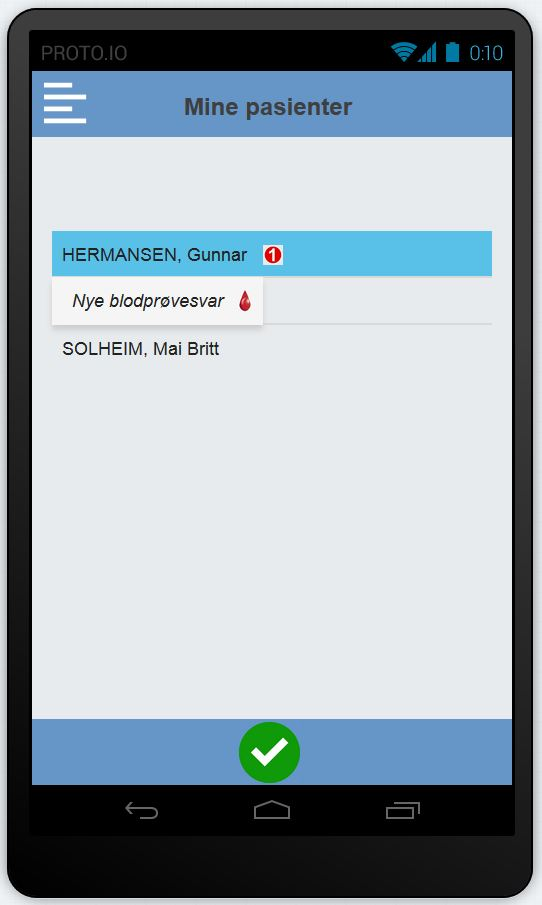
\includegraphics[scale=0.4]{minePasienter.jpg}
\caption{Eksempel på pasientlisten til en sykepleier. Her er det kommet svar på blodprøvende til Hermansen.}
\label{minePasienter}
\end{figure}

\subsubsection{Mine Beskjeder}
Mine beskjeder er en slags sms-lignende tjeneste hvor sykepleierene kan stille hverandre med spørsmål og gi beskjeder som ikke haster. Dette er en mindre forstyrrende og avbrytende måte å kommunisere på, når det ikke er avgjørende med rask respons.

\subsubsection{Kontakter}
Her vises kontaktinformasjon inkludert tilgjengelighet til de sykepleierene som er på jobb. Her skal det være enkelt å få oversikt over alle som er på vakt, og om de er tilgjengelige eller ikke. Dette er ment å brukes blandt annet dersom man har et spørsmål som flere kan svare på. Ved hjelp av kontaktlisten kan man velge den som mest sannsynlig vil bli minst forstyrret av henvendelsen. Ved å trykke på kontakten vil denne automatisk bli oppringt.

\subsubsection{Telefon}
Dette er den vanlige telefonfunksjonen vi kjenner fra vanlige telefoner, og trenger ingen detaljert forklaring.



